\documentclass[11pt]{report}
\usepackage[utf8]{inputenc}
\usepackage[margin=2.0cm]{geometry}
\usepackage{fancyhdr}
\usepackage{xcolor}
\usepackage{minted}
\usepackage{graphicx}
\usepackage[parfill]{parskip}

\title{Digital Engineering\\Lab 2}
\author{Y3890959\\Y3878784}
\date{31st January 2023}

\pagestyle{fancy}
\fancyhead{}
\setlength{\headheight}{14pt}
\fancyhead[L]{Lab 1}
\fancyhead[R]{Y3890959, Y3878784}
\fancyfoot{}
\fancyfoot[L]{Digital Engineering}
\fancyfoot[R]{\thepage}

\makeatletter
\let\ps@plain\ps@fancy 
\makeatother

\setminted {
    fontsize=\footnotesize,
    frame=single,
}

\begin{document}

\maketitle

\chapter*{Task A: Timing Simulation}

\section*{1.1.1 Self-Checking Testbench}
\inputminted{vhdl}{../../Lab2/Lab2.srcs/sim_1/new/algorithm_tb.vhd}

\section*{1.1.2 Behavioural Simulation}
\subsection*{Waveform 1: Global Initialisation/Reset}
\begin{figure}[H]
    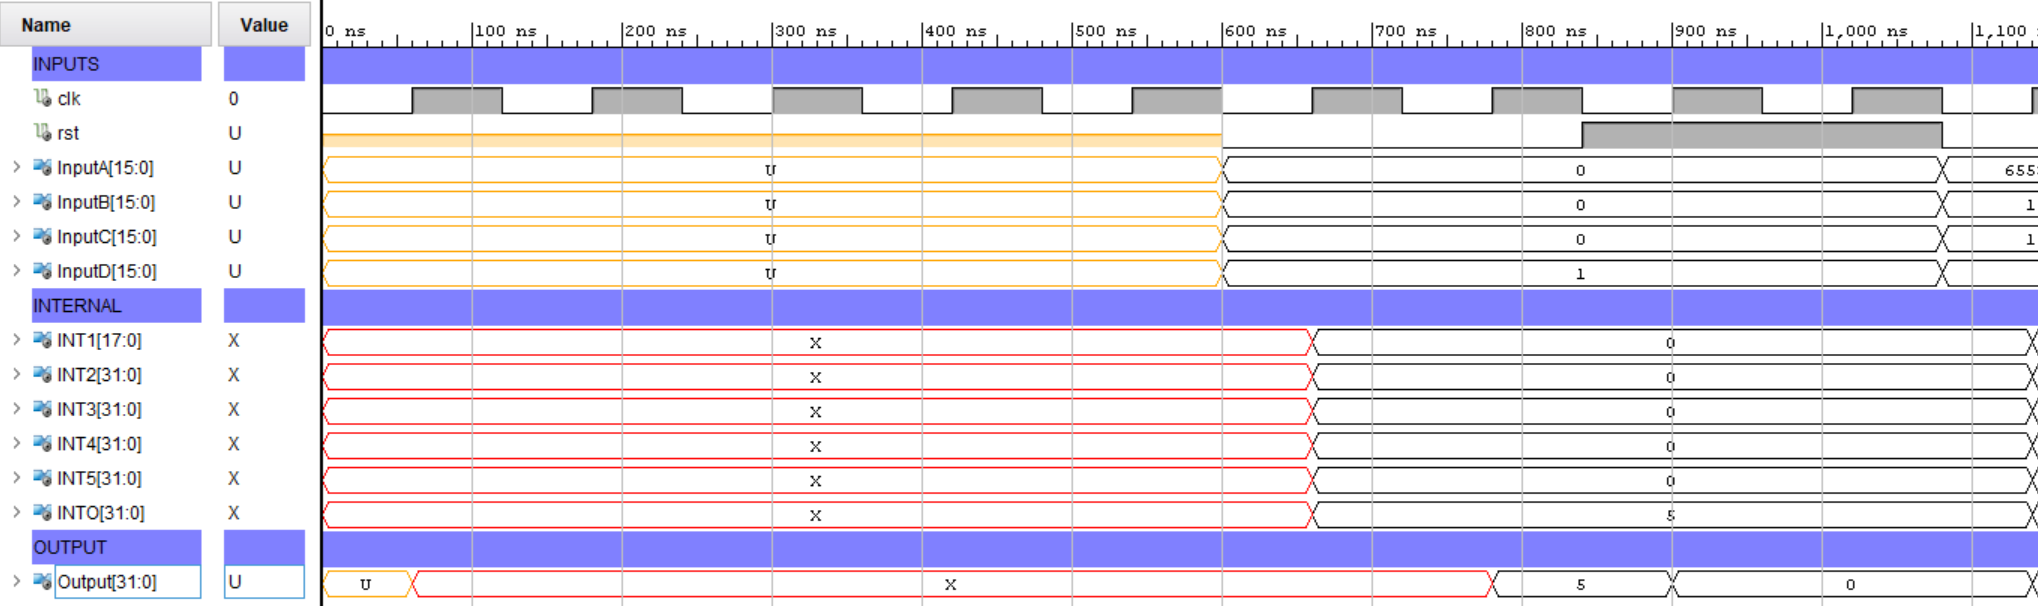
\includegraphics[width=\columnwidth]{Reports/Lab2/Waveforms/120ns_behavioural_global-reset.png}
\end{figure}
\subsection*{Waveform 2: Test Sequence}
\begin{figure}[H]
    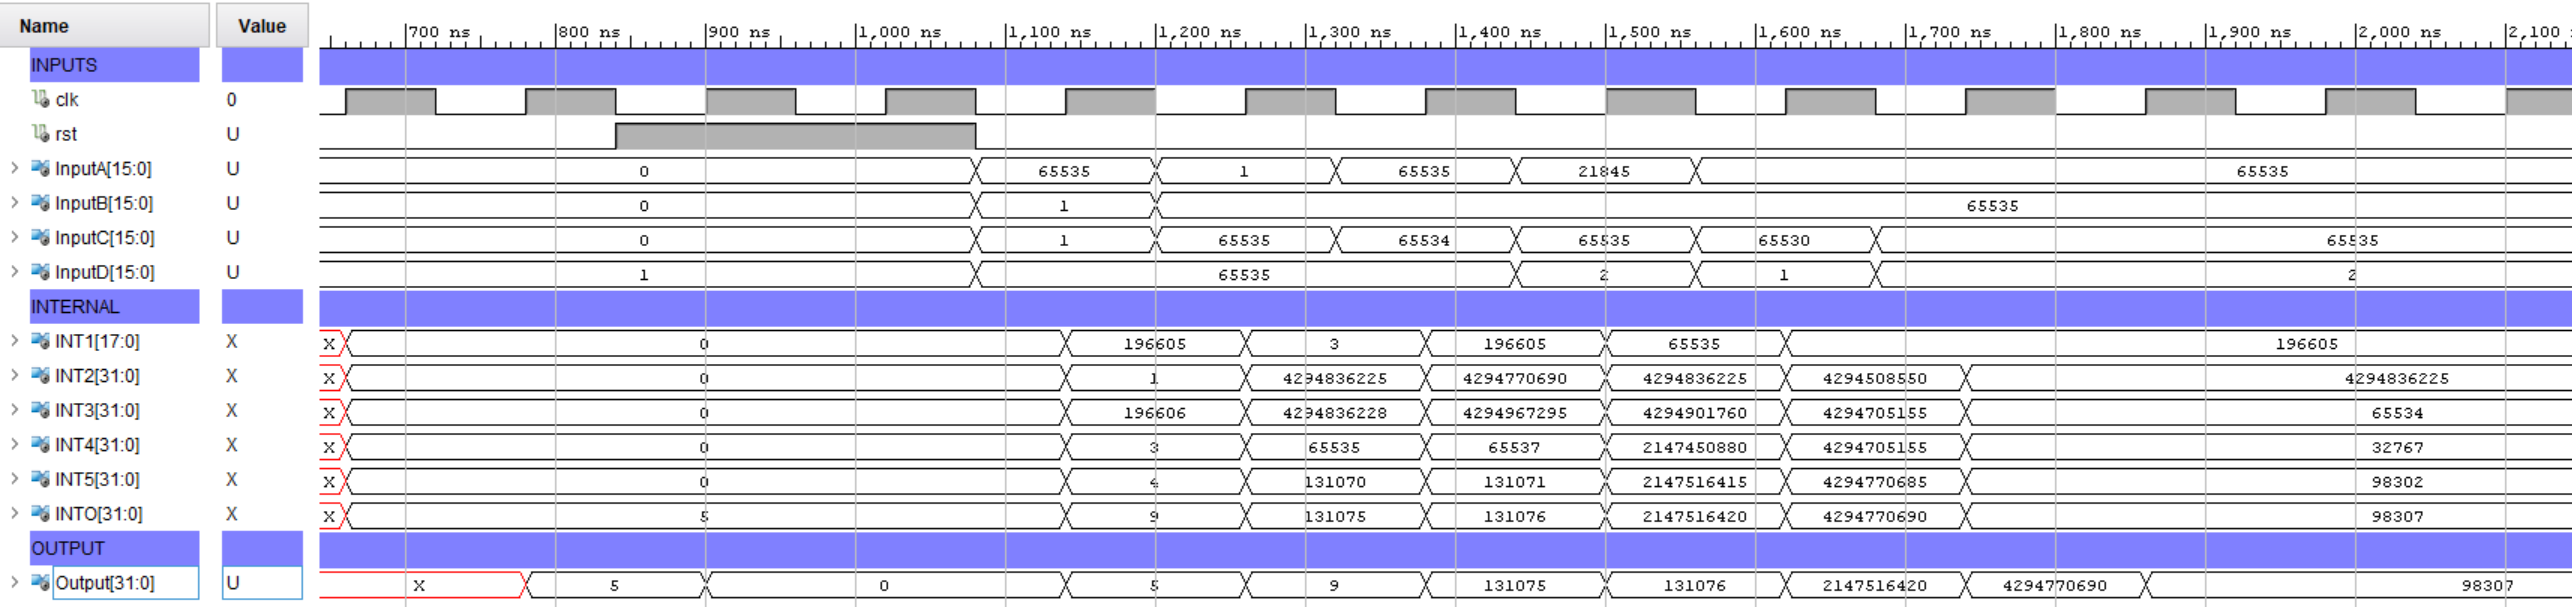
\includegraphics[width=\columnwidth]{Reports/Lab2/Waveforms/120ns_behavioural_test-sequence.png}
\end{figure}
\subsection*{Console Output}
\begin{figure}[H]
    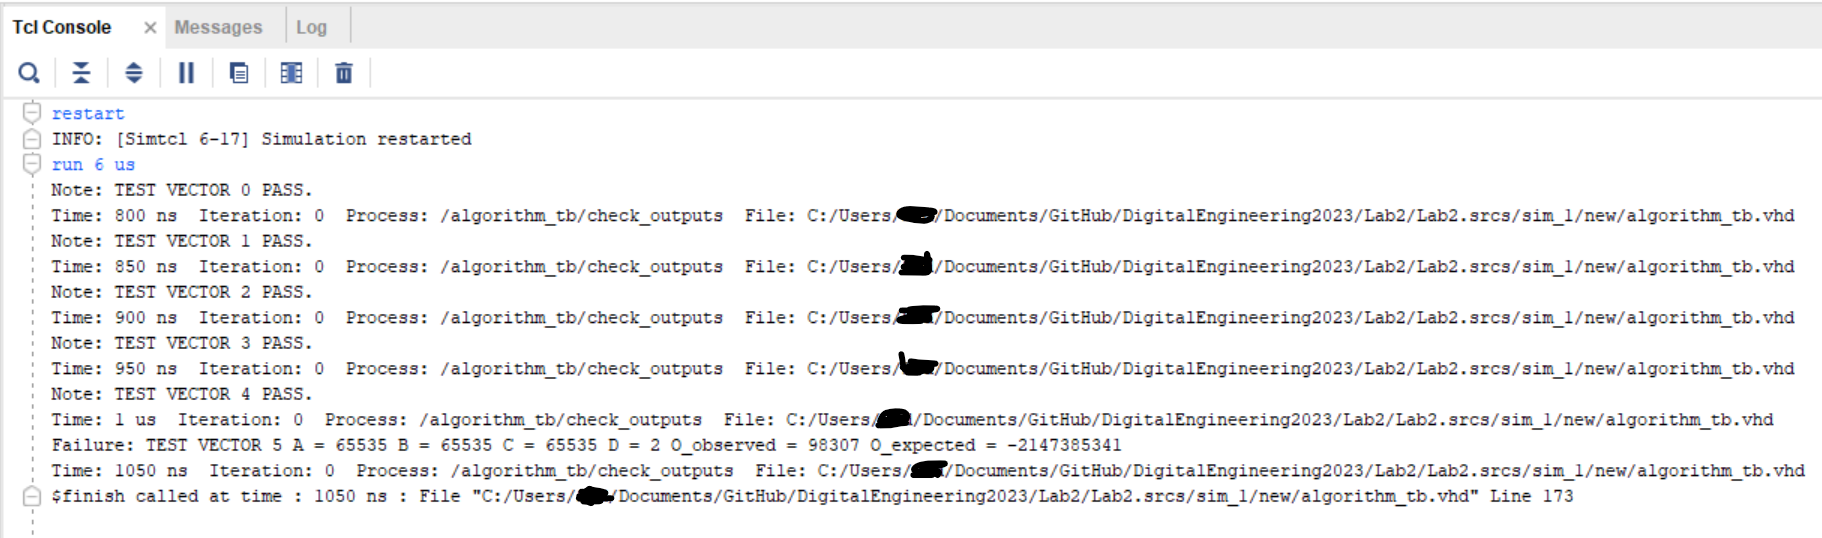
\includegraphics[width=\columnwidth]{Reports/Lab2/Waveforms/120ns_behavioural-console.png}
\end{figure}


\section*{1.1.3 Design Runs - WNS}
\begin{figure}[H]
    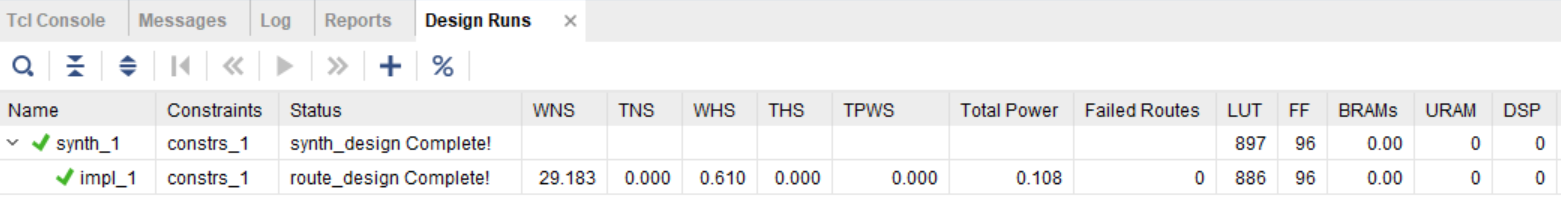
\includegraphics[width=\columnwidth]{Reports/Lab2/Waveforms/design_runs-WNS.png}
\end{figure}
The implementation process consists of 3 steps: `Translate', where the netlist and constraints are merged into an Xilinx design file. `Map', where the design is implemented on the target device. And finally, `place and route', where the components are placed and routes are designed according to the timing constraints. This process incorporates proprietary and classified algorithms that rely on random factors, therefore, the same design will never be implemented twice.

After the `place and route' step is complete, the tools will be able to provide an estimate of all the propagation delays for all signals within the entire device after the `static timing analysis' step. With the timing information, the tools can calculate the `worst negative slack' (WNS).

From the WNS value we got from our implementation, we can run our circuit with a clock signal as fast as 90.817ns, or around 11.01MHz.


\section*{1.1.4 Timing Simulation (120ns Clock)}
\subsection*{Waveform 1: Global Initialisation/Reset}
\begin{figure}[H]
    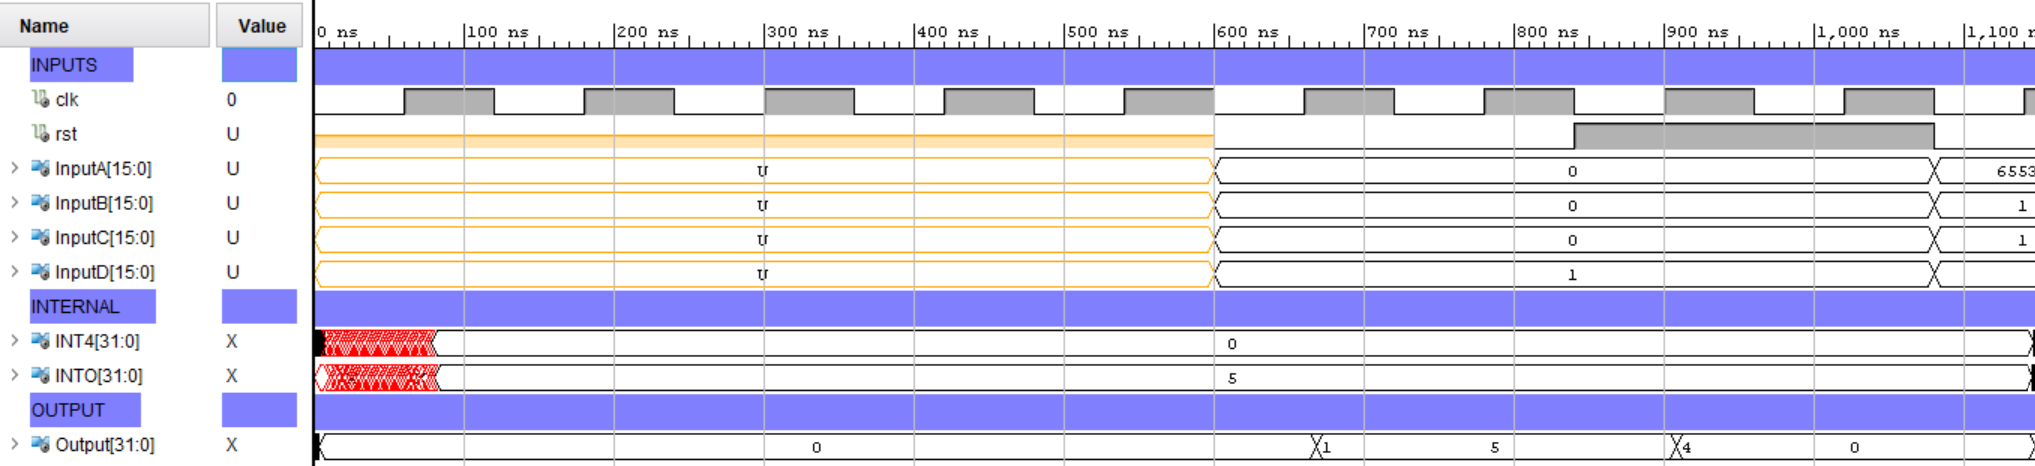
\includegraphics[width=\columnwidth]{Reports/Lab2/Waveforms/120ns_timing_sim-global-reset.png}
\end{figure}
\subsection*{Waveform 2: Test Sequence}
\begin{figure}[H]
    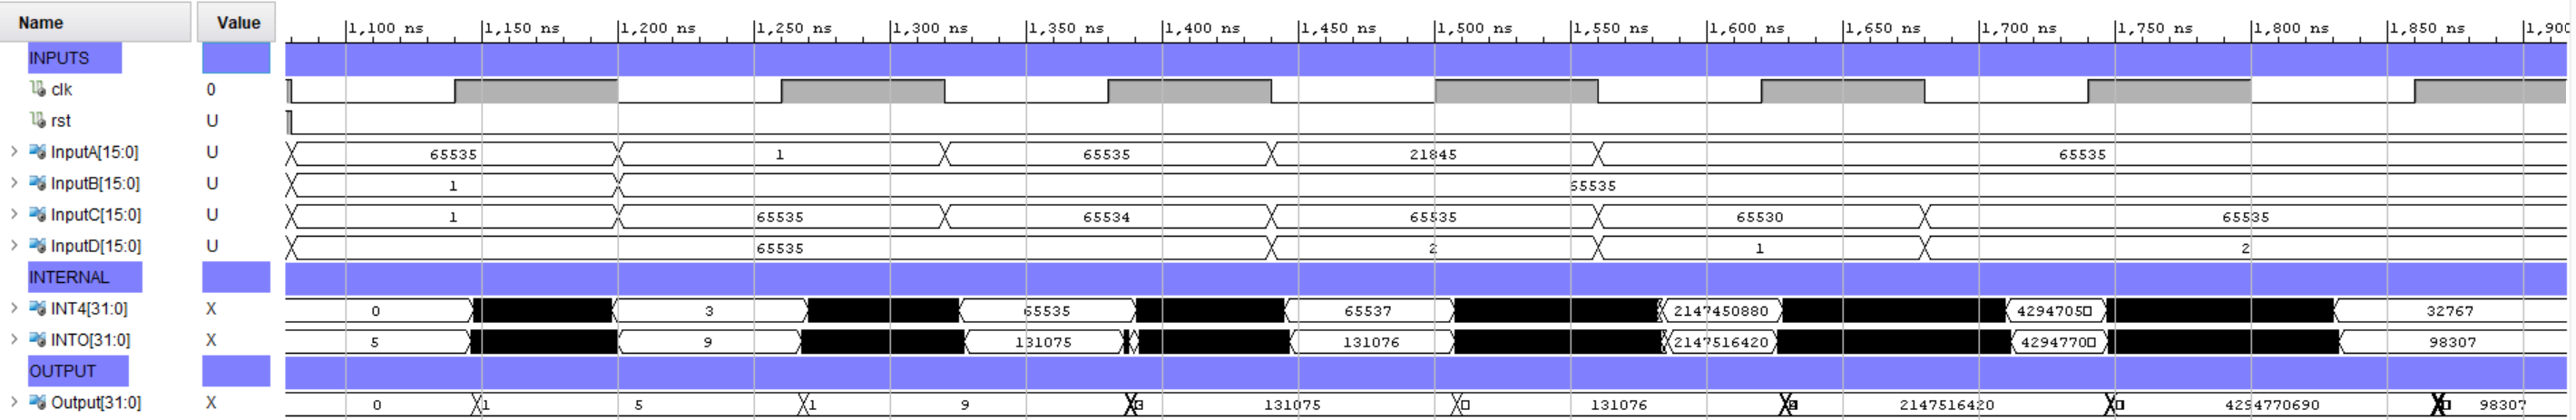
\includegraphics[width=\columnwidth]{Reports/Lab2/Waveforms/120ns_timing_sim-test-sequence.png}
\end{figure}
\subsection*{Console Output}
\begin{figure}[H]
    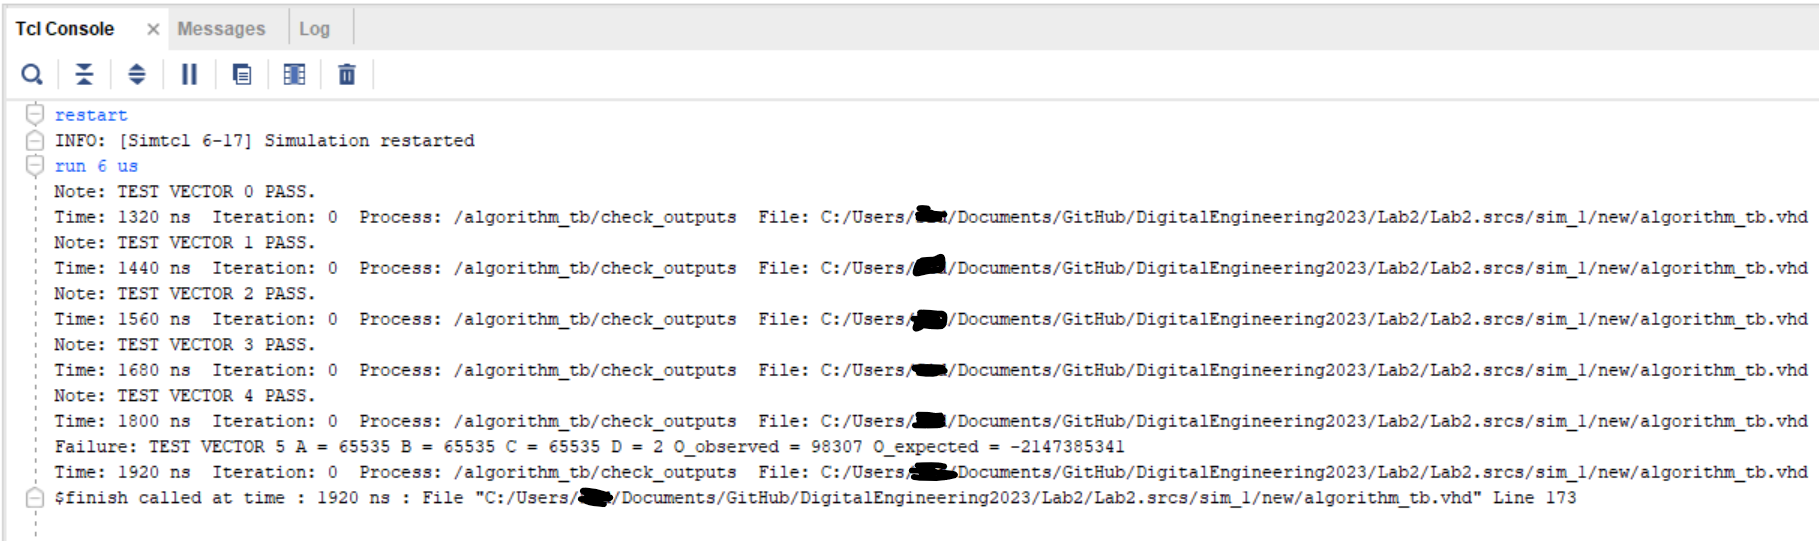
\includegraphics[width=\columnwidth]{Reports/Lab2/Waveforms/120ns_timing_sim-console.png}
\end{figure}


\section*{1.1.5 Timing Simulation (50ns Clock)}
\subsection*{Waveform 1: Global Initialisation/Reset}
\begin{figure}[H]
    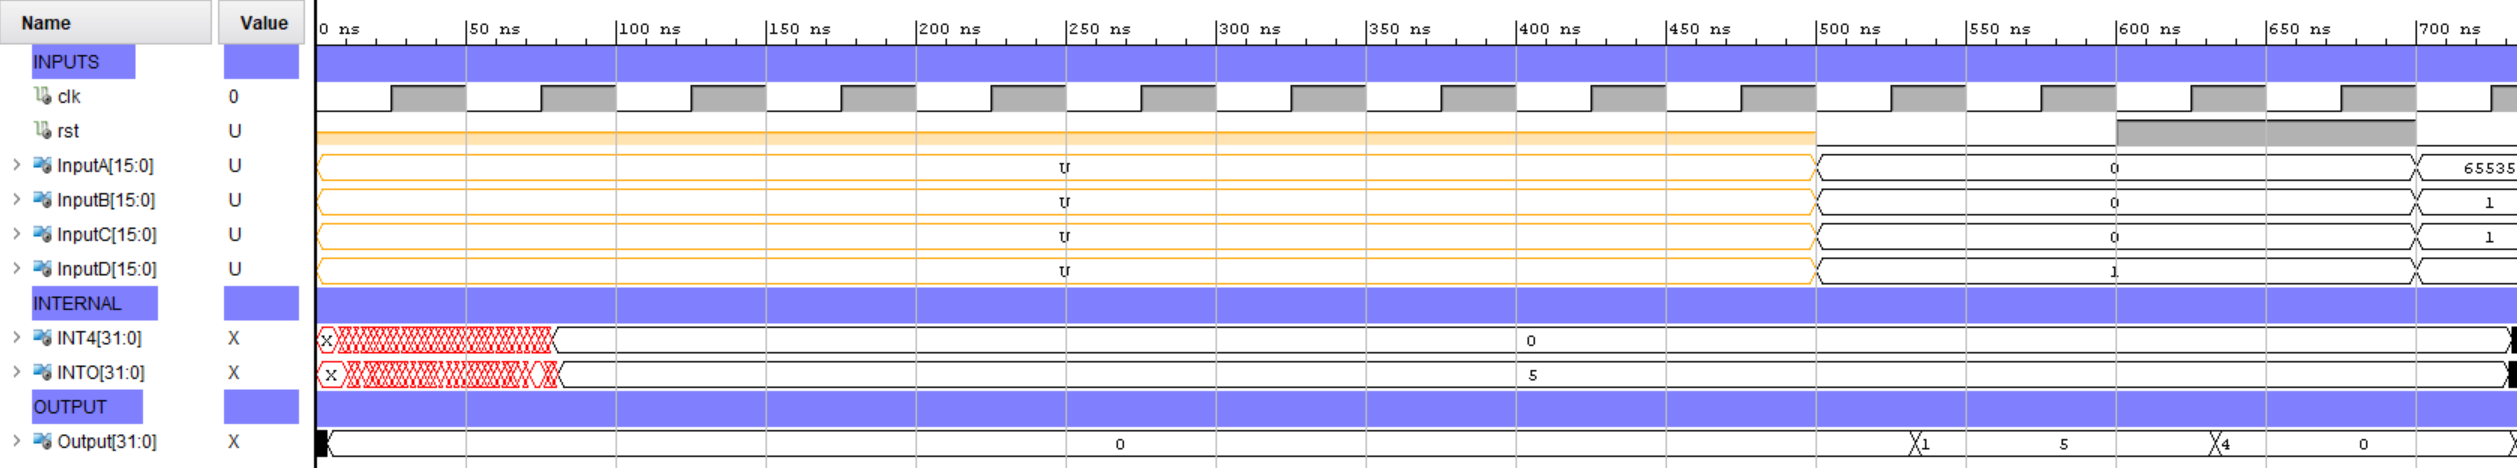
\includegraphics[width=\columnwidth]{Reports/Lab2/Waveforms/50ns_timing_sim-global-reset.png}
\end{figure}
\subsection*{Waveform 2: Test Sequence (Vector \#1-3)}
\begin{figure}[H]
    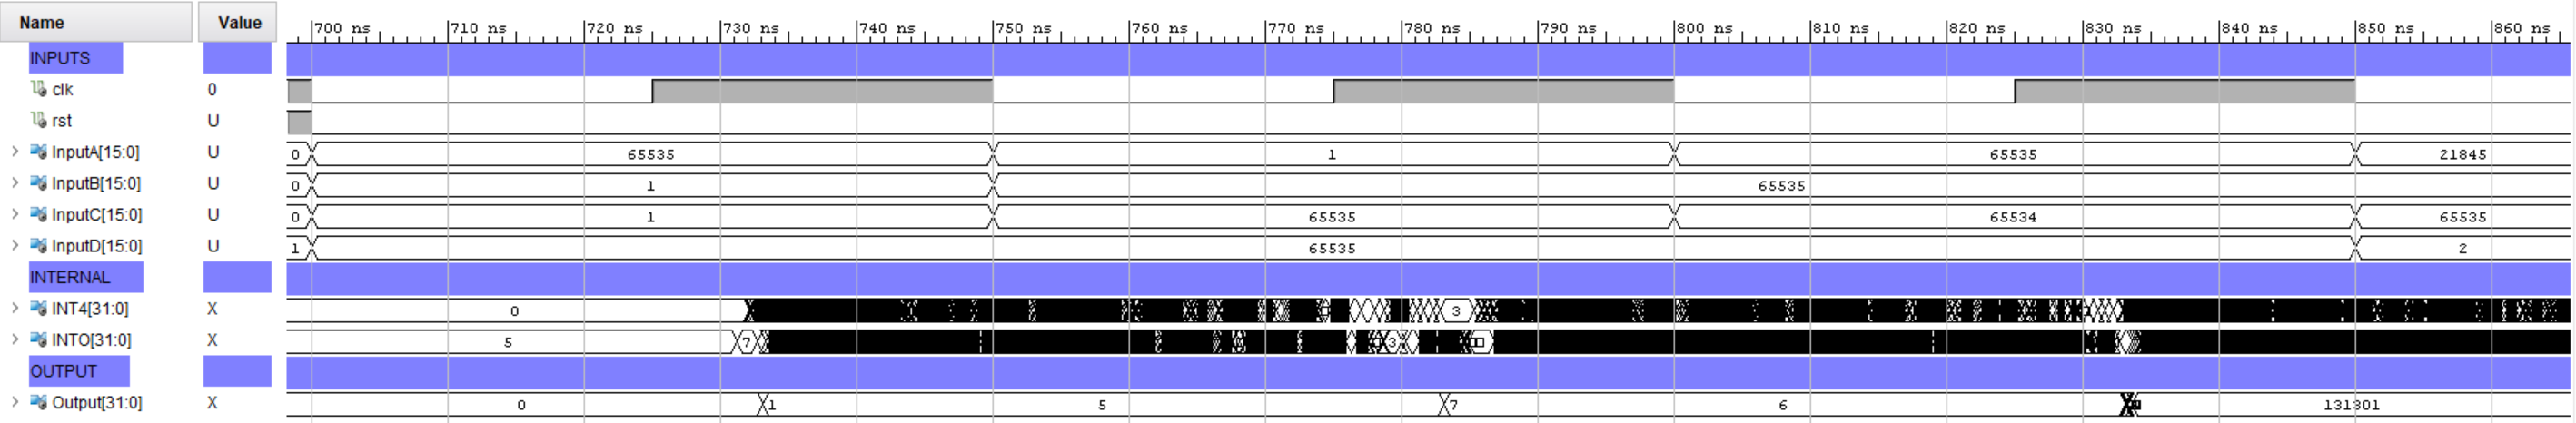
\includegraphics[width=\columnwidth]{Reports/Lab2/Waveforms/50ns_timing_sim-test-sequence-1-3.png}
\end{figure}
\subsection*{Waveform 3: Test Sequence (Vector \#3-6)}
\begin{figure}[H]
    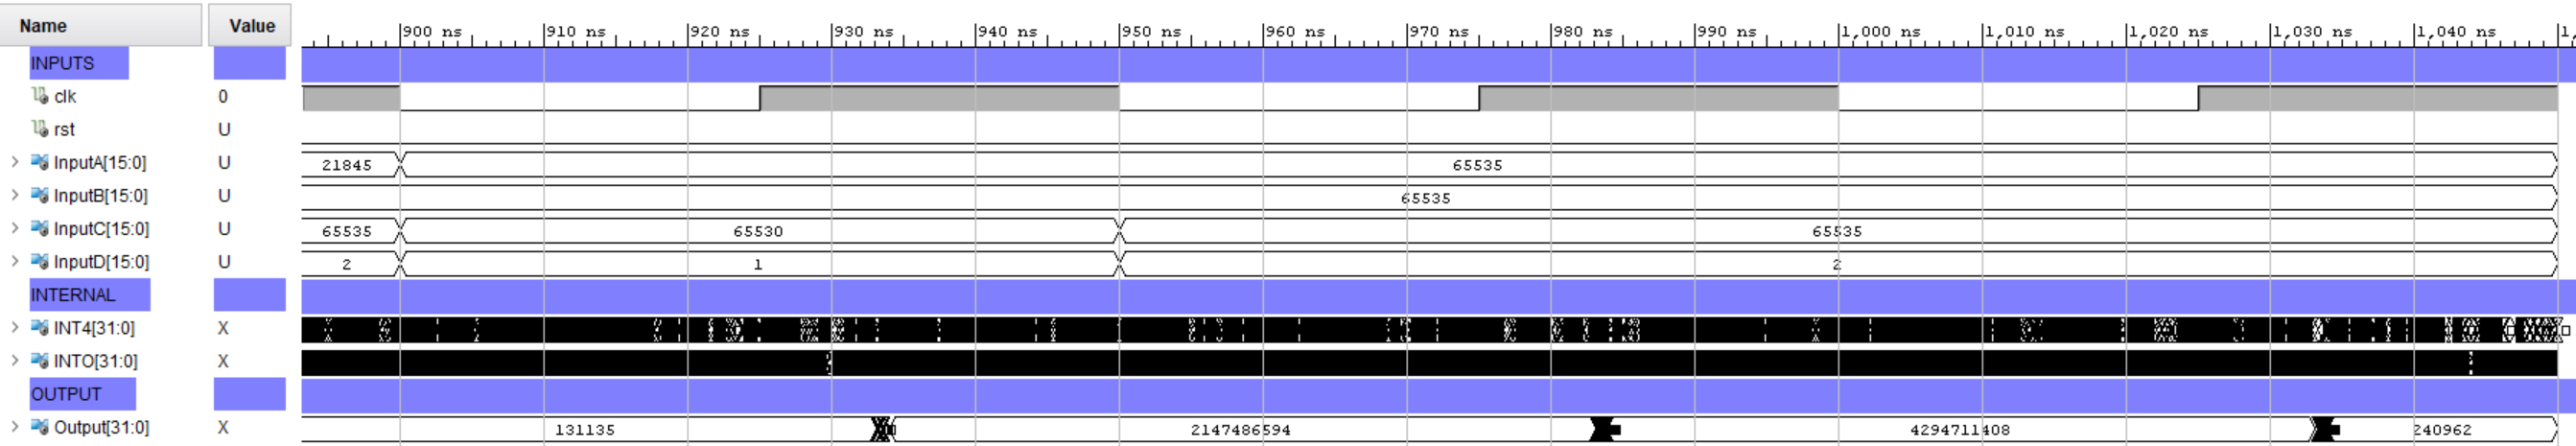
\includegraphics[width=\columnwidth]{Reports/Lab2/Waveforms/50ns_timing_sim-test-sequence-3-6.png}
\end{figure}
\subsection*{Console Output}
\begin{figure}[H]
    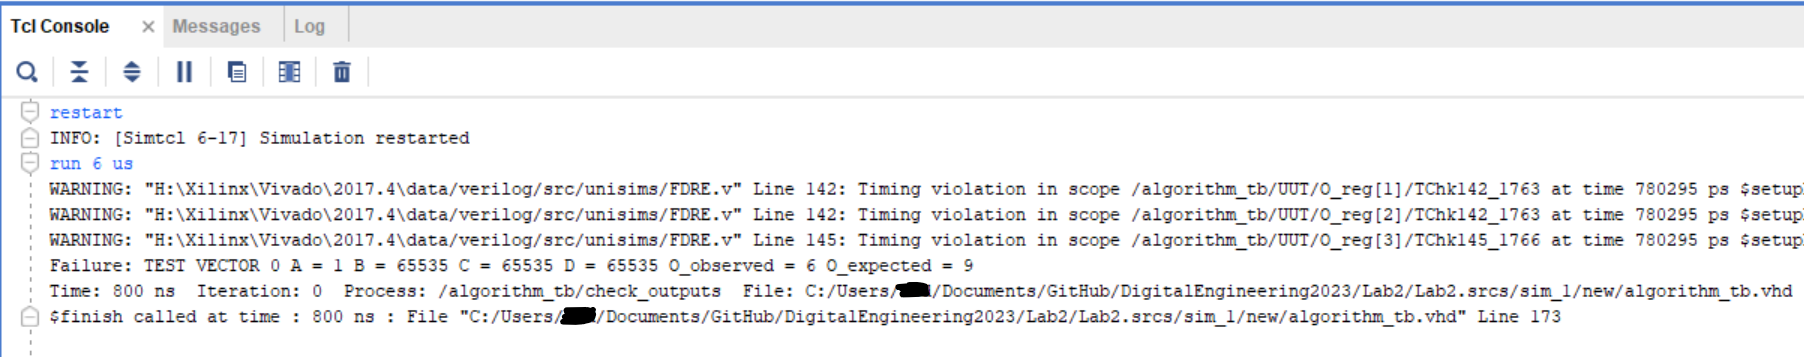
\includegraphics[width=\columnwidth]{Reports/Lab2/Waveforms/50ns_timing_sim-console.png}
\end{figure}


\section*{1.1.6 Analysis of Results}
\subsection*{Question 1}
During the synthesis stage to generate the netlist, the tools will process the project VHDL files to check syntax and optimise designs. Due to this optimisation step, the tools will optimise across all hierarchy levels (unless it's explicitly told not to do so), therefore, hierarchy is often destroyed. 

As the implementation stage needs to be run for the timing simulations, these simulations are based on the netlist. Therefore, we can only see the INT4 and INTO internal signals, all others have been destroyed by the tools for optimisation purposes.

\subsection*{Question 2}
As propagation delays aren't taken into account with a simple behavioural simulation, we can notice everything changes at the exact edge of the clock. The post-implementation timing simulation on the other hand takes into account of these delays, therefore, changes only happen once the signal has propagated and before that, intermediate transient values are produced due to unequal propagation.

Comparing the `INTO' signals, we see that the value changes to the correct one only after half a clock cycle of metastability, this is due to unequal propagation delays. The `Output` signal is slightly delays relative to the rising clock edge, and there seems to be an intermediate transient value, likely caused by the metastability of `INTO'.

\subsection*{Question 3}
In the simulation results from 1.1.4, we say `INTO' metastability lasting only around half a clock cycle, in the waveform from 1.1.5, we see metastability throughout INTO. We can also see the increase in metastability as the simulation progresses; in Waveform 2 (Vector \#1-3), there are a few moments where the value stays fixed for a nanosecond or two, but in Waveform 3 (Vector \#3-6), the output for INTO turns into a dark black rectangle.

The behaviour for the Output signal is also quite consistent with the one from 1.1.4, the only difference being the Output is incorrect (due to the metastable INTO). But we can notice as INTO metastability increases in Waveform 2, there seems to be an increase in metastable transient values between register outputs.


\chapter*{Task B: Tool Optimisations}


\end{document}
